\chapter[The Reluctant Quantum Mechanician]{The Reluctant Quantum Mechanician}\label{chap22}


\Authorline{Sharath Ananthamurthy}

\authinfo{School of Physics, University of Hyderabad}

I met Gowravaram Ramachandran-GR-to his countless students and disciples spread all over here and abroad, during one of my trips back to Mysore from Kanpur, where I had just joined the M.Sc.\ in physics course. Anand, a friend from college days, who'd been bitten by the ``theoretical physics bug", had arranged the meeting at the time. Slightly, over an hour during this chat (that I remember, went on for two! -- apparently GR was famous for this) I already started to regret going away to far-flung places such as Kanpur for pursuing my love for the subject, when such wonderful and inspiring teachers such as the one I was in front of, were to be found right in my town! For one who has always been reluctant to go away anywhere else, being in love with Mysore and the Mysorean life, this meeting only compounded the homesickness I was experiencing in Kanpur. I vividly remember that conversation, with my friend looking on with reverence and a benign smile, while hanging on to every word from GR, casting an occasional glance at me to ensure I was also sufficiently taken in with this intellectual treat. With a sagging enthusiasm to pursuing my school love for physics, the feeling assisted by a cluster of bad teachers (with the exception of one outstanding teacher, Ramesh Chandra) during college days, the above-mentioned friend, with a strong interest in Physics and the Feynman Lectures in Physics in equal measure, had taken it upon himself to get me to the Gangotri Physics Department and hoped to cure me of my uncertainties, through exposure. I recall having experienced time dilation!  A session that lasted two hours seemed in my mind like sheer poetry! In a rather poorly lit room, sat GR surrounded by stacks of books piled up on the table and in corners of the room. He sat in the same position over the entire discussion, where he held a monologue about the polarized states of photons and the modes of radiation with my friend, interspersing this with gentle inquiries about who was teaching me what subjects, at IIT Kanpur. He seemed to know all my teachers from there, and made brief and sharp comments on the significant research contributions of a few of them. He also seemed to know a whole lot of things about the theoretical physics research scene in the country. Two hours later, as I emerged out of his room into the brightly lit quadrangle space of the department, it was like emerging out of a cinema theatre after being in an intense movie experience. 

During the years in high school, I had had the good fortune of being around some persons who were great physics teachers- Professors Srinivasan, at the Yuvaraja College, and Ramesh Chandra, at the Sarada Vilas College, were both presences not only in the class room, but were found attending many cultural events- the evening \textit{sangeetha kacheris} held in the bylanes of Mysore, or at the Centenary Hall of the University, where large numbers from the Mysore neighborhoods would often gather to watch theatre and plays directed and acted in by their friends. Many stories of physics and physicists were heard through the walks back home, most certainly from one of the groups of walkers, each one in loud discussion about the play they had just watched or some other mundane matter. This was in the late seventies and early eighties when no distances seemed too far in Mysore!  It is in these walks that I remember hearing about the discoveries in particle physics, about quantum mechanics and all the excitement in physics. Gangotri was still far away from my mental space, for that was the place where the ``big guys in physics all sat"! I heard over time of the big names, the other teachers at Gangotri, Professors K. N. Sreenivasa Rao, D. Krishnamurthy, the two Sanjeevaiahs - BS and HS, the Gandhian Sanjeevaiah - K. Gopal (or KG), A. V. Gopala Rao;  they were all well-known. The Department by then already could boast of the presence of such luminaries who had once served there, such as Pancharatnam, or Chandrashekar, of the ``liquid crystal" fame. GR had joined in 1973 after a brief stint as Scientific Officer in the company of the formidable G. N. Ramachandran at IISc. With him, the Department experienced a rebirth of sorts of modern quantum mechanics!  I went away to pursuing a Ph.D. in the United States in the eighties. When I returned, and several years later, joined the University of Mysore, in 1996, GR was on the verge of retiring. But the year or so spent in his company, proved once again a treat!

Just a few weeks after I was settling in, he ambled into the little room I shared with a postdoc, Dr.\ Swarna, also his student. He was keen to learn what I had studied for the Ph.D. I explained to him my work, which was in laser spectroscopy. I had set up experiments and investigated atomic collisions and how initial orbital alignment of colliding atoms influence the collisional outcome of energy states. I had carried out measurements of the polarization of the collisionally redistributed radiation, from which we could envision through quantum mechanical models the possible initial and final state alignment of the atomic orbitals with reference to the axis along which the collision occurred. He listened to me with rapt attention, then got up and smiled at me remarking as he left, ``you may have done experiments but you are a theorist at heart"!  I called out to him as he was exiting, `` Sir, but I am an experimental physicist", but he appeared to shrug off my insistence of being recognized as an experimentalist. To this date, his remark has stuck in my mind, and I often think of the sociological implications of this remark, but those thoughts don't have a place here.

Not having been his \textit{shishya} in a direct way, I had the benefit of seeing GR in action only from a distance, in a manner of speaking. The language of quantum mechanics, was what he seemed so fluent in! Like a poet, he seemed to explore its every nuance. And I've seen the magic of this artist performing in research seminars- I sat in initially on the seminars on entangled quantum states that GR's research group had arranged- he could, chalk in one hand, the other at his back, gently holding the baggy terry cot trousers he wore, as if they may fall, unfold and layout to his spellbound audience, result after result elegantly following a general formalism. All this seemed to flow out from the piece of chalk he held in his other hand. Nonstop!  The seminars, of course went way past their time, but we had all been transformed into another world, so mundane affairs such as lunch, or restroom breaks didn't seem necessary. He never carried a lunch box, coming in to the department after a brunch. Not even a cup of coffee would he touch, and his colleagues were all polite enough to not embarrass him by offering anything. 

The next few meetings with GR, happened a few years later in the early 2000, when as a visiting professor at the Indian Institute of Astrophysics in Bangalore, he stepped in to help in a collaboration I had with the late Dr.\ Nagendra, also a former student who formed part of the ``diaspora" of GR-students. We were guiding a Myanmarese doctoral student, Ms.\ Yee Yee Oo, my first, in an astrophysical problem on spectral line formation from stars with varying magnetic fields. Dr.\ Nagendra and I struggled a bit with the quantum mechanical formalism that involved a considerable amount of angular momentum algebra before asking GR to step in. Not only did GR show us elegant ways of dealing with the algebra but also pointed out new avenues that we could explore by considering electric fields in the problem. Collaborations with him led to the publishing of two nice papers in a spectroscopy journal. This is my only formal collaboration with him. I eventually stopped atomic theory calculations and started to build my labs for soft matter research while at Bangalore University where I had since moved. My distance from both GR and Nagendra grew as I became more involved in laboratory research in soft matter. 

The indomitable teacher that he was, GR after retirement missed his greatest love- having students around him. So, I heard he had started classes right at home, gathering interested students who gravitated to physics and who all missed the presence of good teachers in their lives but yearned for one. Over time, a few other enthusiasts would float the ``special short term courses" with GR as their star performer. GR never tired of any opportunity to explain to anyone who came to him with interest, was always there, chalk in hand and ready to deliver the long monologues, building as he went along, a complete picture in front of the newer recruits. I felt quite moved at his enthusiasm and untiring effort, but sad at the same time that institutions no longer could keep him in their fold. But nothing dithered GR. What he needed was a board, chalk, and students.

In my somewhat limited understanding of the perspectives on the theoretical research GR carried out with his students, gathered through my own conversations with him and students of his, has led me to believe that he was a die-hard classicist in his approach. Having mastered the formalism and foundational aspects of quantum mechanics (including field theory), his work was linked to a strong belief and practice of discovery, that one had to explore the formalism deeply to discover the right parts that help in analyzing and explaining a particular physical phenomenon. GR applied this approach, mostly to problems in nuclear and particle physics. This mode of discovering seemed much to do with a belief that ``it's all right there in the texts, one needs to know how to look for and what to look at", to address the problem at hand. This seemed different from the somewhat more messy knowledge construction wherein the formalism may be subject to changes even if slight, here and there, quite often not very clean, sometimes not very thorough even. Such activity needs conversations and discussions with other physicists or people from other disciplines. In these aspects it is my observation that he was reluctant to reach out and interact with the community. The formalism was like the Vedas, with nothing to be added to but simply applied. Many papers emerged out of his skill at applying the formalism, always with remarks and a wry smile, that he was taking part in the new fashion, from remote Mysore.

As the activities in science and the communities of physicists grew in different parts of the world, so did the number of meetings and conferences arranged in different parts of the country. For a man so prolific in publishing, he was reluctant to go anywhere and refused all invited talks. His students did go out, posters tucked away under their arms, or to give Talks about GRs work. But not with GR accompanying them to any meeting! At a time when it became necessary increasingly, to actively publicize one's work through conference travel, here was a physicist who seemed comfortable with the travel that was confined to trips between home and Gangotri!  My guess is that in his personal life, being an orthodox Brahmin and a \textit{swayam paki}, if not for the homemade food cooked by the other householders, forbade travel that involved staying in unfamiliar places. He seemed most comfortable in Mysore, and the University, that made no demands on him by imposing administrative tasks such as Chairmanships, or university administrative positions. It left him alone, to do what he loved most-his single minded physics \textit{tapas}, and teaching.
\vspace{.5cm}

\centerline{\includegraphics[scale=.48]{authorsphotos/Sharath_Ananthamurthy.eps}}

\authbio{Sharath Ananthamurthy}
\bigskip

\noindent
\textbf{Dr.\ Sharath Ananthamurthy} obtained the M.S. in 1988 and Ph.D. in 1993 from the University of Iowa, USA. He joined the Physics Department, Mysore University in 1996. During his stay of two years at Mysore University he had close interaction with Prof.\ Ramachandran and, also later, when Prof.\ Ramachandran moved to IIA, Bangalore. He moved to Physics Department, Bangalore University, in 1998, as a Reader and rose to the position of Professor in 2006. In 2017, Dr.\ Sharath moved to the School of Physics, University of Hyderabad.
